%%
%% This is file `sample-manuscript.tex',
%% generated with the docstrip utility.
%%
%% The original source files were:
%%
%% samples.dtx  (with options: `manuscript')
%% 
%% IMPORTANT NOTICE:
%% 
%% For the copyright see the source file.
%% 
%% Any modified versions of this file must be renamed
%% with new filenames distinct from sample-manuscript.tex.
%% 
%% For distribution of the original source see the terms
%% for copying and modification in the file samples.dtx.
%% 
%% This generated file may be distributed as long as the
%% original source files, as listed above, are part of the
%% same distribution. (The sources need not necessarily be
%% in the same archive or directory.)
%%
%% Commands for TeXCount
%TC:macro \cite [option:text,text]
%TC:macro \citep [option:text,text]
%TC:macro \citet [option:text,text]
%TC:envir table 0 1
%TC:envir table* 0 1
%TC:envir tabular [ignore] word
%TC:envir displaymath 0 word
%TC:envir math 0 word
%TC:envir comment 0 0
%%
%%
%% The first command in your LaTeX source must be the \documentclass command.
%%%% Small single column format, used for CIE, CSUR, DTRAP, JACM, JDIQ, JEA, JERIC, JETC, PACMCGIT, TAAS, TACCESS, TACO, TALG, TALLIP (formerly TALIP), TCPS, TDSCI, TEAC, TECS, TELO, THRI, TIIS, TIOT, TISSEC, TIST, TKDD, TMIS, TOCE, TOCHI, TOCL, TOCS, TOCT, TODAES, TODS, TOIS, TOIT, TOMACS, TOMM (formerly TOMCCAP), TOMPECS, TOMS, TOPC, TOPLAS, TOPS, TOS, TOSEM, TOSN, TQC, TRETS, TSAS, TSC, TSLP, TWEB.
% \documentclass[acmsmall]{acmart}

%%%% Large single column format, used for IMWUT, JOCCH, PACMPL, POMACS, TAP, PACMHCI
% \documentclass[acmlarge,screen]{acmart}

%%%% Large double column format, used for TOG
% \documentclass[acmtog, authorversion]{acmart}

%%%% Generic manuscript mode, required for submission
%%%% and peer review
\documentclass[manuscript,screen,review]{acmart}

\usepackage{todonotes}
%% Fonts used in the template cannot be substituted; margin 
%% adjustments are not allowed.
%%
%% \BibTeX command to typeset BibTeX logo in the docs
\AtBeginDocument{%
  \providecommand\BibTeX{{%
    \normalfont B\kern-0.5em{\scshape i\kern-0.25em b}\kern-0.8em\TeX}}}

%% Rights management information.  This information is sent to you
%% when you complete the rights form.  These commands have SAMPLE
%% values in them; it is your responsibility as an author to replace
%% the commands and values with those provided to you when you
%% complete the rights form.
\setcopyright{acmlicensed}
\copyrightyear{2018}
\acmYear{2018}
\acmDOI{XXXXXXX.XXXXXXX}

%% These commands are for a PROCEEDINGS abstract or paper.
\acmConference[Conference acronym 'XX]{Make sure to enter the correct
  conference title from your rights confirmation emai}{June 03--05,
  2018}{Woodstock, NY}
%
%  Uncomment \acmBooktitle if th title of the proceedings is different
%  from ``Proceedings of ...''!
%
\acmBooktitle{Woodstock '18: ACM Symposium on Neural Gaze Detection,
 June 03--05, 2018, Woodstock, NY} 
\acmISBN{978-1-4503-XXXX-X/18/06}


%%
%% Submission ID.
%% Use this when submitting an article to a sponsored event. You'll
%% receive a unique submission ID from the organizers
%% of the event, and this ID should be used as the parameter to this command.
%%\acmSubmissionID{123-A56-BU3}

%%
%% For managing citations, it is recommended to use bibliography
%% files in BibTeX format.
%%
%% You can then either use BibTeX with the ACM-Reference-Format style,
%% or BibLaTeX with the acmnumeric or acmauthoryear sytles, that include
%% support for advanced citation of software artefact from the
%% biblatex-software package, also separately available on CTAN.
%%
%% Look at the sample-*-biblatex.tex files for templates showcasing
%% the biblatex styles.
%%

%%
%% The majority of ACM publications use numbered citations and
%% references.  The command \citestyle{authoryear} switches to the
%% "author year" style.
%%
%% If you are preparing content for an event
%% sponsored by ACM SIGGRAPH, you must use the "author year" style of
%% citations and references.
%% Uncommenting
%% the next command will enable that style.
%%\citestyle{acmauthoryear}

%%
%% end of the preamble, start of the body of the document source.
\begin{document}

%%
%% The "title" command has an optional parameter,
%% allowing the author to define a "short title" to be used in page headers.
\title{The Name of the Title is Hope}

%%
%% The "author" command and its associated commands are used to define
%% the authors and their affiliations.
%% Of note is the shared affiliation of the first two authors, and the
%% "authornote" and "authornotemark" commands
%% used to denote shared contribution to the research.
\author{Luke Hennessy}
\email{henneslk@dukes.jmu.edu}
\orcid{0009-0000-2924-4437}
% \orcid{0009-0009-1072-00132}
\author{Michael C. Stewart}
\email{stewarmc@jmu.edu}
\orcid{0000-0002-8833-7833}
\affiliation{%
  \institution{James Madison University}
  \streetaddress{701 Carrier Dr.}
  \city{Harrisonburg}
  \state{Virginia}
  \country{USA}
  \postcode{22807}
}

%%
%% By default, the full list of authors will be used in the page
%% headers. Often, this list is too long, and will overlap
%% other information printed in the page headers. This command allows
%% the author to define a more concise list
%% of authors' names for this purpose.
\renewcommand{\shortauthors}{Trovato and Tobin, et al.}

%%
%% The abstract is a short summary of the work to be presented in the
%% article.
\begin{abstract}
\todo{Luke write abstract}
\end{abstract}

%%
%% The code below is generated by the tool at http://dl.acm.org/ccs.cfm.
%% Please copy and paste the code instead of the example below.
%%
\begin{CCSXML}
<ccs2012>
 <concept>
  <concept_id>00000000.0000000.0000000</concept_id>
  <concept_desc>Do Not Use This Code, Generate the Correct Terms for Your Paper</concept_desc>
  <concept_significance>500</concept_significance>
 </concept>
 <concept>
  <concept_id>00000000.00000000.00000000</concept_id>
  <concept_desc>Do Not Use This Code, Generate the Correct Terms for Your Paper</concept_desc>
  <concept_significance>300</concept_significance>
 </concept>
 <concept>
  <concept_id>00000000.00000000.00000000</concept_id>
  <concept_desc>Do Not Use This Code, Generate the Correct Terms for Your Paper</concept_desc>
  <concept_significance>100</concept_significance>
 </concept>
 <concept>
  <concept_id>00000000.00000000.00000000</concept_id>
  <concept_desc>Do Not Use This Code, Generate the Correct Terms for Your Paper</concept_desc>
  <concept_significance>100</concept_significance>
 </concept>
</ccs2012>
\end{CCSXML}

\ccsdesc[500]{Do Not Use This Code~Generate the Correct Terms for Your Paper}
\ccsdesc[300]{Do Not Use This Code~Generate the Correct Terms for Your Paper}
\ccsdesc{Do Not Use This Code~Generate the Correct Terms for Your Paper}
\ccsdesc[100]{Do Not Use This Code~Generate the Correct Terms for Your Paper}

%%
%% Keywords. The author(s) should pick words that accurately describe
%% the work being presented. Separate the keywords with commas.
\keywords{Do, Not, Us, This, Code, Put, the, Correct, Terms, for,
  Your, Paper}

%% A "teaser" image appears between the author and affiliation
%% information and the body of the document, and typically spans the
%% page.
\begin{teaserfigure}
  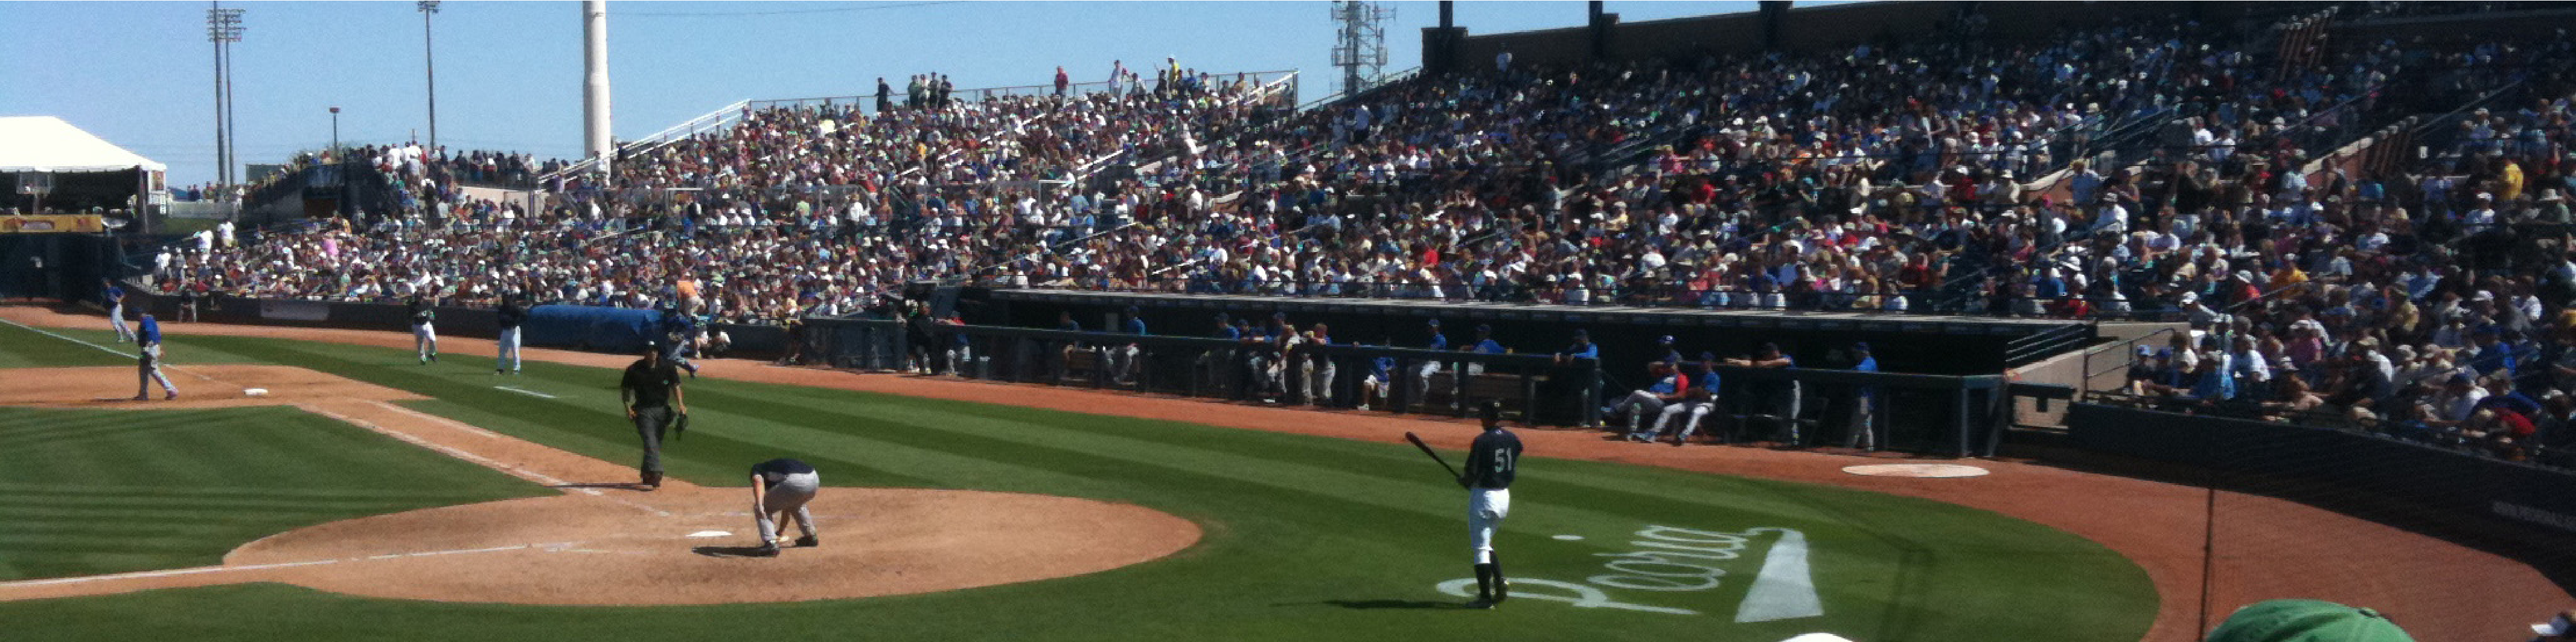
\includegraphics[width=\textwidth]{sampleteaser}
  \caption{Seattle Mariners at Spring Training, 2010.}
  \Description{Enjoying the baseball game from the third-base
  seats. Ichiro Suzuki preparing to bat.}
  \label{fig:teaser}
\end{teaserfigure}

\received{20 February 2007}
\received[revised]{12 March 2009}
\received[accepted]{5 June 2009}

%%
%% This command processes the author and affiliation and title
%% information and builds the first part of the formatted document.
\maketitle



% \begin{itemize}
%     \item USA context: students in cs are a homogeneous bunch (white dudes of relative privilege)
%     \item in primary and secondary education, ``tracking'' prematurely includes/excludes students from some electives/resources/opportunities such CS
%     \item perhaps more kinds of people should have opportunity to learn CS/be introduced in an appropriate way
%     \item perhaps such people would be interested in continuing in CS if they had been exposed properly
%     \item students in instrumental music education courses have a better demographic correlation to their schools' overall demographic profile than those in CS
%     \item what on-ramps into CS might interest students in music ed and simultaneously complement their IME curriculum
%     \item we propose that introducing activities that teach computational thinking and programming and early computer science concepts in the context of instrumental music education activities helps
%     \item 
% \end{itemize}

\section{Introduction}
In the USA context, students in computer science (CS) often represent a homogeneous group, primarily comprising white cishet men with relative privilege. This homogeneity is perpetuated by early educational practices, such as 'tracking,' which can prematurely include or exclude students from certain electives, resources, and opportunities, including CS education. There is a growing recognition that a more diverse range of students should have the opportunity to learn CS and be introduced to it in an appropriate manner. It is plausible that if more people from underrepresented groups were invited to CS education in culturally appropriate and relevant and metacognitively accessible ways, they might develop a sustained interest in the field. Interestingly, students enrolled in instrumental music education (IME) courses exhibit a demographic correlation closer to their schools' overall demographic profile compared to those in CS. Therefore, exploring avenues that can attract students from music education backgrounds to CS, while complementing their IME curriculum, holds promise. We propose integrating activities that teach computational thinking, programming, and early CS concepts within the context of instrumental music education activities as a means to achieve this goal.

% Make more of a case for integration (not just last sentence)
    % Prior work has proven effect and pedagogically sound
    
\subsection{Committee Members}
\begin{itemize}
    \item Michael Stewart, chair
    \item Chris Johnson %\hyperlink{https://deltaphone.twodee.org/}{deltaphone} motivated this, PL, CSEd, CT, HCI with direct manipulation, web apps
    \item Philip Riley

\end{itemize}





% Lukes ORC ID: https://orcid.org/0009-0000-2924-4437


% Ben's project: https://docs.google.com/document/d/1WyLFhY3qPPJs0PLBUmwPXh3xyHusXpcguVUZpO1Tqb0/edit#heading=h.f0w418mo4s2m 



% in what context are you working
% state of IME and HCI and CT around this stuff

    


\section{Related Work}

% report contrasting demographics between CS in public schools vs. music education in the same
% report that integrating CT into other subjects is an area of exploration/inquiry/study, seems like some promise
% discuss direct manipulation interfaces and block programming success for new programmers


In this section, we review literature 

\subsection{Computational Thinking in Education}
In the 1980s,~\citet{papert1980mindstorms} wished for a future where ``to think like a computer" would be considered an ordinary component of thinking skills (p. 155). In line with this,~\citet{wing2006computationalthinking} argues that Computational Thinking (CT) is not just a programming skill, but a daily life skill. According to~\citet{otero2020computational}, CT ``is closely associated with the efforts to convey a systematic and well-structured way of solving problems" (p. 130).~\citet{tatar2017protoCT} describe CT as the principle of ``using elements easily recognizable to computer scientists as computer science, that is, creating algorithms and meta-level descriptions of code, coding, engaging in explicit acts of structure creation, structured top-down problem solving, and so forth" (p. 65). While CT may be defined as elements that are, ``recognizable to computer scientists as computer science'' it is clear that CT includes concepts and  skills that are useful to a wide range of disciplines and problems. CT may be a skill that employs, i.e., abstraction, decomposition, generalisation and evaluation~\cite{selby2013computational}, with the goal to identify patterns, lay connections and ultimately problem-solve. 
% use the concept of proto-computational thinking but maybe use another type of definition like critical thinking (critical thinking is probably part of computational thinking) -> Michael does not necessarily value the name 'proto-computational thinking'
% argument: people (from maybe low-SES) are scared off by CS because they think it is 'difficult', 'only for nerds', 'only for the smartest people'

% what kind of different types of representations are there? In music we have all kinds of note schemes, even depending on what instrument you play it may be different

% Question to answer: why would representing the music in different kinds of structures\representations suddenly make students convinced that they can do CS as well?
% - explain the thought process (maybe some psychology behind it)
% - explain the steps that are taken by the student 

% currently the higher-level argument in the grant is kind of missing. 

\todo{Meagan: Need to review how CT is currently employed across the country. Do we want to argue that schools typically employ CT over PCT?}

\todo{Argue that PCT would be better over general CT to improve equity and engagement with music+CS in diverse groups?}

Although the term CT is relatively new, the practice of teaching CT has been around in education for many years, albeit under different terms~\cite{czerkawski2015exploring}, i.e., procedural thinking~\cite{papert1980mindstorms}, operational thinking, .... One of the earliest known examples of introducing CT to education is during an introductory programming course by Alan Perlis in 1962 at Carnegie Mellon University--then Carnegie Institute of Technology~\cite{perlis1962computer}. In various education systems, CT is being introduced in school curricula simply under labels such as `Computing', `Digital Technologies', and `Computer Science'~\cite{duncan2015pilot, heintz2016reviewofmodels, hubwieser2015global}. However, the introduction of CT in school curricula raises several concerns \cite{tatar2017protoCT}. For our purposes the most relevant is the fact that school curricula tend to be full, and introducing another subject poses the risk of impairing the notion of offering students a `rounded education'~\cite{bell2018integrating}.

1. there's success integrating it in other courses/disciplines

2. we note that many other disciplines have more proportionate representation of all demographics than computer science

3. we also want tot take an integrated approach


% % summary of Michael's article, note citations
% \begin{itemize}
%     \item Computational Thinking: "using elements easily recognizable to computer scientists as computer science, that is, creating algorithms and meta-level descriptions of code, coding, engaging in explicit acts of structure creation, structured top-down problem solving, and so forth. (65)"
%     \item Actions taken in programming spaces, cognition, and even physical action in computer science-related concepts
%     \item CT is controversial but important. Many questions? who needs to learn and why? What disciplines must be focused on and when?
%     \item The direct approach to teaching CT is not always successful when it comes to equity. More affluent schools and students are the ones with the ability and the ones who are more likely to take advantage of the opportunity. This fits with the general preexisting inequality and observed gap between high-income and low-income students for all subjects. (page 64-65 examples of CT already used) 
%     \item Teams4Youth project: description, success, limitations (65)
    
% \end{itemize}
% % basic lit review
% \todo{stewart}
% Search terms:
% \begin{itemize}
%     \item Stewart please do the work
% \end{itemize}


\section{Purpose}
% what you're doing

The purpose of this project is to introduce computational thinking to instrumental education students (like those in middle school band and orchestra classes). Our approach will be to integrate new activities into MusicCPR. MusicCPR is a niche Learning Management System for band and orchestra classes. MusicCPR is implemented as a web application and continues an iterative design and development process as part of its participatory design process including current in-service and pre-service instrumental music educators and music education researchers as co-designers.

MusicCPR currently has ``Creativity'' activities that task the student with composing a musical score (see figure) \todo{make this figure}. As part of this project, we will design and develop new versions of the existing Creativity activities. In the new versions, we will add a block-based programming interface. Deciding which block language to use, and exactly what the user experience with the blocks should be is part of this project's effort. In the interest of illustrating the design space, we now provide a possible implementation.

\subsection{Possible Implementation}
% 

\textbf{Implementation Questions:}
\begin{itemize}
    \item What language should code blocks be translated to? (Python, Previously existing teaching language, Pseudo Code?)
    \item How many steps should there be in the gradual introduction of- and expectation to use/interact with- programming blocks? e.g. 3-step plan students will be assigned 3 pieces of repertoire in sequence in musiccpr: 
    \begin{itemize}
        \item student completes all activities as they are right now in musiccpr for 1 piece of repertoire.
        \item when doing compose for the 2nd piece they will see blocks appear corresponding to the authoring they're doing, perhaps be asked some guided inquiry questions about the blocks
        \item when doing 3rd piece's compose activity, they might be asked to manipulate the blocks
    \end{itemize}
    \item How should the users compose their score? (FlatIO?, etc.)
    \item Does each portion of the project (Code blocks, music score creation, translation) need to be implemented in separate steps, or should work be done on all parts in tandem?
    \item How much Fall time should be spent on research before implementation should begin?
\end{itemize}

\subsection{Block Programming for Music Composition}


% Research and develop software to introduce more students to computational thinking.
 % MusicCPR could be a good platform to expose students to programming and computer science-related ideas. 
% \end{itemize}


\subsection{Research Methods}
\begin{itemize}
    \item Early prototype have music people (maybe Matt test?)
    \item second wizard of OZ with music teachers?
    \item actual students?
\end{itemize}
%  tentative schedule/timeline
\subsection{Fall 2024}
Build the programming blocks and Features (ideally this would be a bit iterative and participatory)



\textbf{Preliminary Implementation Timeline}



% Generator for tables: https://www.tablesgenerator.com/#
\begin{table}[h]
\begin{tabular}{@{}ll@{}}
\toprule
\textbf{Week}                 & \textbf{Goal}                               \\ \midrule
Week 1 (August 26 - 30) & Literature and Market Review      \\
Week 2 (Sep 2 - 6)   & Instructional Design Questions    \\
Week 3 (Sep 9 - 13)  & Instructional Design Questions    \\
Week 4 (Sep 16 - 20) & Discuss Features and Design for Accessibility/Usability \\
Week 5 (Sep 23 - 27) & Project R\&D                      \\
Week 6 (Sep 30 - Oct 4) & Project R\&D                     \\
Week 7 (Oct 7 - 11)  & Project R\&D                      \\ \midrule
\textbf{Fall Break Oct 16 - 20} &                                \\ \midrule
Week 8 (Oct 21 - 25) & Software Development and Start Recruitment process \\
Week 9 (Oct 28 - Nov 1) & Software Development and Recruitment \\
Week 10 (Nov 4 - 8)  & Software Development and Recruitment \\
Week 11 (Nov 11 - 15) & Software Development and Recruitment \\
Week 12 (Nov 18 - 22) & Software Development and Tutorial Creation \\ \midrule
\textbf{Thanksgiving Break Nov 23 - Dec 1} &                   \\ \midrule
Week 13 (Dec 2 - 6)  & Communicate with participants and Address Onboarding Issues \\ \midrule
\textbf{Winter Break Dec 16 - Jan 19} &                           \\ \midrule
Week 14 (Jan 20 - 24) & Data Collection and Analysis and Begin Writing Process\\
Week 15 (Jan 27 - 31) & Data Collection and Analysis       \\
Week 16 (Feb 3 - 7)   & Data Collection and Analysis       \\
Week 17 (Feb 10 - 14) & Data Collection and Analysis       \\ \midrule
Week 18 (Feb 17 - 21) & Create Presentation and Finish Writing Paper \\
Week 19 (Feb 24 - 28) & Create Presentation and Write Paper \\
Week 20 (March 3 - 7) & Create Presentation and Write Paper \\
Week 21 (March 10 - 14) & Create Presentation and Write Paper \\ \midrule
\textbf{Spring Break March 17 - 21)} & Project Completion Goal  \\ \midrule
\end{tabular}
\end{table}




\subsection{Spring 2025}
Have people use it (they should have earlier, but this will be more specifically a broader audience than your co-designers or design informants)

The primary objective of this thesis project is to complement the existing work on MusicCPR with new features that introduce computational thinking in a more familiar context than as a standalone course.
In the United States, many more students have access to instrumental music education than to computer science or computational thinking education.
The students who have access to computer science and computational thinking education opportunities tend to belong to demographics that experience disproportionate unearned privilege in comparison to a school's overall demographic profile.
By developing activities in MusicCPR that introduce computational thinking, we have the opportunity to increase access to computational thinking education.
This might support the students in their primary task (composing music for their instrumental music course) in addition to providing opportunities for students who may not have otherwise had access to experience computational thinking education.
This could broaden participation in computing education by groups that are currently underrepresented.
To study the potential for increasing access and opportunity to various students, we must collect student demographic and experience data:
\begin{enumerate}
    \item race
    \item class
    \item gender
    \item past/current experience with computing education
\end{enumerate}

% Have you ver done programming activity in or out of school?
% computer science class in the school (informal vs formal education)
% camp, etc.
% level of interest 

% Steal stuff from grant proposal shared in Luke google drive



With the project's main objective being the introduction of computational thinking to more students with an additional goal of increasing participation in courses by a group of students who more accurately represent the demographics of the school. Relevant demographic information of participating students such as gender, race, and socio-economic background should be collected in order to assess the success of this part of the objective. This data should also be used to compare against the overall demographics of the school. 

A number of quantitative assessments can be administered for additional analysis like pre and post program assessments to measure knowledge of computer concepts, additional tests for music compositional aptitude, as well as classroom analytics like participation, attendance, and retention. Qualitative surveys and questionnaires could be used to gauge both student and teacher feedback in addition to recording potential interest or disinterest in computer science and music composition further into the future of their academic career. 

The comparison to already existing `Creativity' activities within MusicCPR would provide a benchmark for assessing how these new features impact student engagement and learning outcomes. By evaluating both sets of activities under similar conditions, we can determine whether the proposed innovations offer significant improvements in terms of user interaction, creative output, and overall effectiveness within the program. While comparing these new ideas to the existing `Creativity' activities within MusicCPR would provide valuable insights into their relative impact on student engagement and learning outcomes, such an analysis may extend beyond the scope of this project due to time constraints. However, this could be an area for future research, allowing for a more comprehensive evaluation of the program's overall effectiveness.

%%
%% The acknowledgments section is defined using the "acks" environment
%% (and NOT an unnumbered section). This ensures the proper
%% identification of the section in the article metadata, and the
%% consistent spelling of the heading.
\begin{acks}
To Robert, for the bagels and explaining CMYK and color spaces.
\end{acks}

%%
%% The next two lines define the bibliography style to be used, and
%% the bibliography file.
\bibliographystyle{ACM-Reference-Format}
\bibliography{sample-base}

%%
%% If your work has an appendix, this is the place to put it.
\appendix




\end{document}
\endinput
%%
%% End of file `sample-authordraft.tex'.
